%//==============================--@--==============================//%
\section{Equações de Maxwell}
\label{sec:maxwell-eq}

É necessário um conjunto de quatro vetores para descrever os fenómenos do campo eletromagnético:
\begin{itemize}
    \item[] o campo elétrico, $\mathbf{E}$ (unidades: V/m, volt por metro)
    \item[] o campo de indução magnética, $\mathbf{B}$ (unidades: T, tesla)
    \item[] o campo de deslocamento elétrico, $\mathbf{D}$ (unidades: C/m$^2$, coulomb por metro quadrado)
    \item[] o campo magnético, $\mathbf{H}$ (unidades: A/m, ampère por metro)
\end{itemize}

Para fenómenos eletromagnéticos variáveis no tempo consideraram-se as equações de Maxwell:
$$
    \left\{
    \begin{aligned}%
        \nabla \times \mathbf{E} &= -\dfrac{\partial \mathbf{B}}{\partial t} 
        & &\qquad\text{\small (Lei de Indução)} \\
        \nabla \cdot \mathbf{D} &= \rho_{ext} 
        & &\qquad\text{\small (Lei de Gauss)} \\
        \nabla \times \mathbf{H} &= \mathbf{J}_{ext} + \dfrac{\partial \mathbf{D}}{\partial t} 
        & &\qquad\text{\small (Lei de Ampère com a correção de Maxwell)} \\
        \nabla \cdot \mathbf{B} &= 0 
        & &\qquad\text{\small (Lei de Gauss para o magnetismo)}
    \end{aligned}
    \right.
$$
As quantidades $\rho_{ext}$ $[$C/m$^3]$ e $\mathbf{J}_{ext}$ $[$A/m$^2]$ representam a densidade de carga volumétrica e a densidade de corrente elétrica (fluxo de carga) de quaisquer cargas externas (ou seja, excluindo quaisquer cargas e correntes de polarização induzidas no meio).

As densidades de carga e corrente, $\rho_{ext}$ e $\mathbf{J}_{ext}$, podem ser consideradas como as fontes dos campos eletromagnéticos. Em problemas de propagação de ondas, estas densidades estão localizadas no espaço; por exemplo, estão restritas a fluir numa antena. Os campos elétricos e magnéticos gerados são irradiados a partir destas fontes e podem propagar-se para grandes distâncias até às antenas recetoras.

Longe de geradores (\textit{sources}), i.e., em regiões do espaço livres de fontes (\textit{source-free regions}), as equações de Maxwell tomam uma forma mais simples, em que se considera que $\rho_{ext} = 0$ e $\mathbf{J}_{ext} = 0$.


O mecanismo qualitativo pelo qual as equações de Maxwell originam campos eletromagnéticos que se propagam pode ser visualizado com o seguinte exemplo:

\begin{figure}[H]
    \centering
    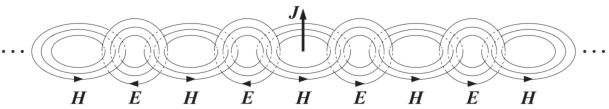
\includegraphics[width=0.7\linewidth]{img/1/Propagacao-de-ondas.pdf}
    \caption{Propagação do campo eletromagnético~\cite{orfanidis2008electromagnetic}}
\end{figure}

\begin{check}
    Uma corrente $\mathbf{J}$ que varia no tempo numa antena linear gera um campo magnético $\mathbf{H}$ circulante e também variável no tempo. Este campo magnético, através da lei de Faraday, origina um campo elétrico $\mathbf{E}$ circulante, que, segundo a lei de Ampère, gera um campo magnético, e assim por diante. Os campos elétricos e magnéticos interligados propagam-se para longe da fonte de corrente.
\end{check}

%//==============================--@--==============================//%
\subsection{Conservação de Carga}

Maxwell adicionou o termo da corrente de deslocamento à lei de Ampère para garantir a conservação da carga. De facto, ao tomarmos a divergência de ambos os lados da lei de Ampère e usando a lei de Gauss $\nabla \cdot \mathbf{D} = \rho$, obtemos:
$$ 
    \nabla \cdot (\nabla \times \mathbf{H}) = \nabla \cdot \mathbf{J}_{ext} + \frac{\partial}{\partial t}(\nabla \cdot \mathbf{D}) = \nabla \cdot \mathbf{J}_{ext} + \frac{\partial \rho_{ext}}{\partial t} 
$$
Usando a identidade vetorial $\nabla \cdot (\nabla \times \mathbf{H}) = 0$, obtemos a forma diferencial da lei de conservação da carga:
$$ 
    \boxed{\frac{\partial \rho_{ext}}{\partial t} + \nabla \cdot \mathbf{J}_{ext} = 0} \quad \text{(conservação da carga)} 
$$

%//==============================--@--==============================//%
\section{Relações Constitutivas e Meios Materiais}

As densidades de fluxo elétrico e magnético, $\mathbf{D}$ e $\mathbf{B}$, estão relacionadas com as intensidades de campo $\mathbf{E}$ e $\mathbf{H}$ através das chamadas \textit{relações constitutivas}, cuja forma precisa depende do material no qual os campos existem. No vácuo, assumem a sua forma mais simples:
$$
    \boxed{%
        \begin{aligned}
            \mathbf{D} &= \epsilon_{0} \mathbf{E} \\
            \mathbf{B} &= \mu_{0} \mathbf{H}
        \end{aligned}
    }
    \quad\rightarrow\quad
    \left\{
    \begin{aligned}
        \epsilon_{0} &\approx 8.854 \cdot 10^{-12} \; [\text{F/m}]\\
        \mu_{0} &\approx 4\pi \cdot 10^{-7} \; [\text{H/m}]
    \end{aligned}\right.
$$
onde $\epsilon_{0}$ e $\mu_{0}$ são a permitividade e permeabilidade do vácuo, respetivamente.

A partir de $\epsilon_{0}$ e $\mu_{0}$, podemos definir outras duas constantes, nomeadamente, a velocidade da luz e a impedância característica do vácuo:
$$
    \boxed{%
        c_0 = \frac{1}{\sqrt{\epsilon_{0} \mu_{0}}} = 3 \cdot 10^8 \; [\text{m/s}], 
        \quad
        \eta_0 = \sqrt{\frac{\mu_{0}}{\epsilon_{0}}} \approx 120\pi\; [\Omega]
    }
$$

A forma mais simples das relações constitutivas é para dielétricos simples, homogéneos e isotrópicos, e para materiais magnéticos:
$$
    \boxed{%
    \begin{aligned}
        \mathbf{D} &= \epsilon \mathbf{E} \\
        \mathbf{B} &= \mu \mathbf{H}
    \end{aligned}
    }
$$
Esta relação é tipicamente válida para frequências mais baixas. A permitividade $\epsilon$ e a permeabilidade $\mu$ estão relacionadas com as suscetibilidades elétrica e magnética dos materiais, i.e.,
$$
    \boxed{%
    \begin{aligned}
        \epsilon &= \epsilon_{0} (1 + \chi)  \\
        \mu &= \mu_{0} (1 + \chi_m)
    \end{aligned}
    }
$$
As suscetibilidades $\chi$ e $\chi_m$ são medidas das propriedades de polarização elétrica e magnética do material. Por exemplo, temos para a densidade do fluxo elétrico:
$$
    \mathbf{D} = \epsilon \mathbf{E} = \epsilon_{0} (1 + \chi) \mathbf{E} = \epsilon_{0} \mathbf{E} + \epsilon_{0} \chi \mathbf{E} = \epsilon_{0} \mathbf{E} + \mathbf{P}
$$
onde $\mathbf{P} = \epsilon_{0} \chi \mathbf{E}$ representa a polarização dielétrica do material, isto é, o momento dipolar elétrico médio por unidade de volume. Num material magnético, temos:
$$
    \mathbf{B} = \mu_0 (\mathbf{H} + \mathbf{M}) = \mu_0 (\mathbf{H} + \chi_m \mathbf{H}) = \mu_0 (1 + \chi_m) \mathbf{H} = \mu \mathbf{H}
$$
onde $\mathbf{M} = \chi_m \mathbf{H}$ é a magnetização, isto é, o momento magnético médio por unidade de volume. A velocidade da luz no material e a impedância característica são:
$$
    c = \frac{1}{\sqrt{\mu \epsilon}} , \quad \eta = \sqrt{\frac{\mu}{\epsilon}}
$$
A permitividade e a permeabilidade relativa, e o índice de refração de um material são definidos por:
$$
    \epsilon_{r} = \frac{\epsilon}{\epsilon_{0}} = 1 + \chi, \quad \mu_{r} = \frac{\mu}{\mu_0} = 1 + \chi_m, \quad n = \sqrt{\epsilon_{r} \mu_{r}}
$$
Podemos relacionar a velocidade da luz e a impedância do material com os correspondentes valores no vácuo:
$$
c = \frac{1}{\sqrt{\mu \epsilon}} = \frac{1}{\sqrt{\mu_0 \epsilon_{0} \epsilon_{r} \mu_{r}}} = \frac{c_0}{\sqrt{\epsilon_{r} \mu_{r}}} = \frac{c_0}{n}
$$
$$
    \eta = \sqrt{\frac{\mu}{\epsilon}} = \sqrt{\frac{\mu_0 \mu_{r}}{\epsilon_{0} \epsilon_{r}}} = \eta_0 \sqrt{\frac{\mu_{r}}{\epsilon_{r}}} = \eta_0 \frac{\mu_r}{n} = \eta_0 \frac{n}{\epsilon_r}
$$
Para um material não magnético, temos $\mu = \mu_0$ ou $\mu_r = 1$, e a impedância simplifica para $\eta = \eta_0/n$.

%//==============================--@--==============================//%

De uma forma mais geral, as relações constitutivas podem ser não homogéneas, anisotrópicas, não lineares, dependentes da frequência (dispersivas) ou todas as anteriores. 

Em \textit{materiais não homogéneos}, a permitividade depende da localização dentro do material:
$$
    \mathbf{D}(\mathbf{r},t) = \epsilon(\mathbf{r}) \mathbf{E}(\mathbf{r},t)
$$

Em \textit{materiais anisotrópicos}, $\epsilon$ depende das direções $x$, $y$, $z$ e as relações constitutivas podem ser escritas em forma de matriz (ou tensor):
$$
    \begin{bmatrix}
        D_x \\
        D_y \\
        D_z \\
    \end{bmatrix} =
    \begin{bmatrix}
        \epsilon_{xx} & \epsilon_{xy} & \epsilon_{xz} \\
        \epsilon_{yx} & \epsilon_{yy} & \epsilon_{yz} \\
        \epsilon_{zx} & \epsilon_{zy} & \epsilon_{zz} \\
    \end{bmatrix}
    \begin{bmatrix}
        E_x \\
        E_y \\
        E_z \\
    \end{bmatrix}
$$
A anisotropia é uma propriedade inerente da estrutura atómica/molecular do dielétrico. Também pode ser causada pela aplicação de campos externos.

Em \textit{materiais não lineares}, $\epsilon$ pode depender da magnitude  $E$ do campo elétrico aplicado na forma:
$$
    \mathbf{D} = \epsilon (E) \mathbf{E}, \quad \text{onde} \quad \epsilon(E) = \epsilon + \epsilon_2 E^2 + \epsilon_3 E^3 + \ldots
$$
Uma consequência típica da não linearidade é causar harmónicas de ordem superior.

Materiais com uma constante dielétrica dependente da frequência, $\epsilon(\omega)$, são referidos como \textit{dispersivos}. A dependência da frequência surge porque quando um campo elétrico variável no tempo é aplicado, a resposta de polarização do material \underline{não pode ser instantânea}. Tal resposta dinâmica pode ser descrita pela relação constitutiva convolucional (e causal):
$$
    \mathbf{D}(\mathbf{r}, t) = \int_{-\infty}^{t} \epsilon(t - t') \mathbf{E}(\mathbf{r}, t') dt'
$$
que se torna multiplicativa no domínio da frequência:
$$
    \underline{\mathbf{D}}(\mathbf{r}, \omega) = \epsilon(\omega) \underline{\mathbf{E}}(\mathbf{r}, \omega)
$$
Na realidade, todos os materiais são dispersivos. Contudo, $\epsilon(\omega)$ tipicamente exibe uma forte dependência de $\omega$ apenas para certas frequências. 


%//==============================--@--==============================//%
\subsection{Eletrodinâmica Macroscópica}

As densidades $\rho_{ext}$ e $\mathbf{J}_{ext}$ representam as cargas e correntes externas ou livres num meio material. A polarização induzida $\mathbf{P}$ e a magnetização $\mathbf{M}$ podem ser tornadas explícitas nas equações de Maxwell através das relações constitutivas:
$$
    \mathbf{D} = \epsilon_0 \mathbf{E} + \mathbf{P}, \quad \mathbf{B} = \mu_0 (\mathbf{H} + \mathbf{M})
$$
Assim, podemos escrever as equações de Maxwell em termos dos campos $\mathbf{E}$ e $\mathbf{B}$:
$$
    \begin{aligned}
        \nabla \times \mathbf{E} &= -\frac{\partial \mathbf{B}}{\partial t}
        &
        \nabla \times \mathbf{B} &= \mu_0 \epsilon_0 \frac{\partial \mathbf{E}}{\partial t} + \mu_0 \mathbf{J}_{ext} + \mu_0 \frac{\partial \mathbf{P}}{\partial t} + \mu_0 \nabla \times \mathbf{M}
        \\
        \nabla \cdot \mathbf{E} &= \frac{1}{\epsilon_0} (\rho - \nabla \cdot \mathbf{P})
        &
        \nabla \cdot \mathbf{B} &= 0
    \end{aligned}
$$
Identificamos assim as densidades de corrente e carga devido à polarização do material como: 
$$
    \mathbf{J}_{pol} = \frac{\partial \mathbf{P}}{\partial t}, \quad \rho_{pol} = -\nabla \cdot \mathbf{P}
$$
Da mesma forma, a quantidade $\mathbf{J}_{mag} = \nabla \times \mathbf{M}$ pode ser identificada como a corrente de magnetização. 

Para um meio dielétrico e condutor (e.g., plasma), acresce-se à lei de Ampère a componente $\mathbf{J}_{cond} = \sigma \mathbf{E}$. As densidades totais de corrente e carga, num meio material genérico, são:

$$
    \mathbf{J}_{tot} 
    = 
    \eqnmarkbox[blue]{free1}{\mathbf{J}_{ext}} + \eqnmarkbox[red]{bound1}{\mathbf{J}_{cond} + \mathbf{J}_{pol} + \mathbf{J}_{mag}}
    = 
    \eqnmarkbox[blue]{free2}{\mathbf{J}_{ext}} + \eqnmarkbox[red]{bound2}{\sigma \mathbf{E} + \frac{\partial \mathbf{P}}{\partial t} + \nabla \times \mathbf{M}}
$$
\annotatetwo{above, label below}{free1}{free2}{macro currents}
\annotatetwo{below, label above}{bound1}{bound2}{micro currents}

\vspace*{-0.75em}
$$
    \rho_{tot} = \rho + \rho_{pol} = \rho - \nabla \cdot \mathbf{P}
$$
e podem ser considerados como as fontes dos campos.

\begin{check}
    Estas relações satisfazem as equações de Maxwell macroscópicas,
    $$
        \boxed{%
            \nabla \times \mathbf{E} = -\frac{\partial \mathbf{B}}{\partial t},
            \quad
            \nabla \times \mathbf{H} = \mathbf{J}_{ext} + \sigma \mathbf{E} + \dfrac{\partial \mathbf{D}}{\partial t}
        }
    $$
    A resposta material (dipolar) está "oculta" nos vetores de polarização e magnetização $\mathbf{P}$ e $\mathbf{M}$, respetivamente.
\end{check}

%//==============================--@--==============================//%
\subsection{Modelos Simples de Dielétricos e Condutores}

Um modelo simples para as propriedades dielétricas de um material pode ser obtido considerando o movimento de um eletrão ligado na presença de um campo elétrico aplicado. À medida que o campo elétrico tenta separar o eletrão do núcleo positivamente carregado, cria-se um momento de dipolo elétrico. A média deste momento de dipolo ao longo do volume do material dá origem a um momento de dipolo macroscópico por unidade de volume.

Um modelo simples para a dinâmica do deslocamento $\mathbf{r}$ do eletrão ligado é o seguinte (onde $\dot{\mathbf{r}} = d\mathbf{r}/dt$):
$$
    m\ddot{\mathbf{r}} = e \mathbf{E} - k\mathbf{r} - m\Gamma\dot{\mathbf{r}}
    \quad \text{(modelo Drude-Lorentz)}
$$
onde assumimos que o campo elétrico está a atuar na direção $\mathbf{r}$ e que existe uma força restauradora tipo-mola devido à ligação do eletrão ao núcleo, e uma força de atrito proporcional à velocidade do eletrão.

A constante da mola $k$ está relacionada à frequência de ressonância da mola pela relação $\omega_0 = \sqrt{k/m}$, ou $k = m\omega_0^2$. Assim, podemos reescrever a equação como:
$$
    \boxed{%
        \ddot{\mathbf{r}} + \Gamma\dot{\mathbf{r}} + \omega_0^2 \mathbf{r} = \frac{e}{m} \mathbf{E}
    }
$$
O termo friccional $\Gamma\dot{\mathbf{r}}$ surge de colisões que tendem a desacelerar o eletrão. O parâmetro $\Gamma$ é uma medida da taxa de colisões por unidade de tempo, e, portanto, $\tau = 1/\Gamma$ representará o tempo médio entre colisões.

\begin{check}
    A ideia básica deste modelo é que o campo elétrico aplicado tende a separar cargas positivas de cargas negativas, criando assim um momento de dipolo elétrico. Neste sentido, o modelo contém as características básicas de outros tipos de polarização em materiais.
\end{check}


%//==============================--@--==============================//%
\subsubsection{Meio Dielétrico Dispersivo}

O campo elétrico aplicado pode ter qualquer dependência temporal. Em particular, se assumirmos que é sinusoidal com frequência $\omega$, então, a equação modelo terá a solução $\mathbf{r} = \Re\{\mathbf{\underline{r}} e^{j\omega t}\}$, onde o fasor $\mathbf{\underline{r}}$ deve satisfazer:
$$
    -\omega^2 \mathbf{\underline{r}} + j\omega \Gamma \mathbf{\underline{r}} + \omega_0^2 \mathbf{\underline{r}} = \frac{e}{m} \mathbf{\underline{E}}
    \implies
    \mathbf{\underline{r}} = \frac{e/m}{\omega_0^2 - \omega^2 + j\omega\Gamma}\, \mathbf{\underline{E}}
$$
Podemos encontrar assim a polarização por unidade de volume no domínio da frequência, $\mathbf{\underline{P}}$. Supondo que existem $N$ dipolos elementares por unidade de volume e admitindo o momento de dipolo elétrico individual $\mathbf{\underline{p}} = e\mathbf{\underline{r}}$, vem:
$$
    \mathbf{\underline{P}} = N \mathbf{\underline{p}} = Ne\mathbf{\underline{r}} = \frac{Ne^2}{m} \frac{1}{\omega_0^2 - \omega^2 + j\omega\Gamma}\, \mathbf{\underline{E}} \equiv \epsilon_0 \chi(\omega) \mathbf{\underline{E}}
$$
A densidade do fluxo elétrico será: $\mathbf{\underline{D}} = \epsilon_0 \mathbf{\underline{E}} + \mathbf{\underline{P}} = \epsilon_0 (1 + \chi(\omega)) \mathbf{\underline{E}} = \epsilon(\omega) \mathbf{\underline{E}}$, onde a permitividade efetiva $\epsilon(\omega)$ é:
$$
    \boxed{%
        \epsilon(\omega) = \epsilon_0 \left( 1 + \frac{\omega_p^2}{\omega_0^2 - \omega^2 + j\omega\Gamma} \right)
    }
    \quad \text{onde} \quad
    \omega_p = \sqrt{\frac{N e^2}{\epsilon_0 m}} \quad \text{(frequência de plasma)}
$$
este modelo para $\epsilon(\omega)$ é conhecido como um ``dielétrico de Lorentz''.

\begin{warning}
    As partes real e imaginária de $\epsilon(\omega)$ caracterizam as propriedades \emph{refrativas} e \emph{absorventes} do material. Por convenção, definimos a parte imaginária com o sinal negativo (porque usamos a dependência temporal $e^{j\omega t}$):
    $$
        \epsilon(\omega) = \epsilon'(\omega) - j\epsilon''(\omega), \quad \text{onde}
    $$
    $$
            \epsilon'(\omega) = \Re\{\epsilon(\omega)\} = \epsilon_0 + \frac{\epsilon_0\omega_p^2(\omega_0^2 - \omega^2)}{(\omega_0^2 - \omega^2)^2 + \Gamma^2\omega^2} 
            \qquad\qquad
            \epsilon''(\omega) = -\Im\{\epsilon(\omega)\} = \frac{\epsilon_0\omega_p^2\Gamma\omega}{(\omega_0^2 - \omega^2)^2 + \Gamma^2\omega^2}
    $$
    \vspace{-1.5em}
    \begin{figure}[H]
        \centering
        \begin{subfigure}[b]{0.45\linewidth}
            \centering
            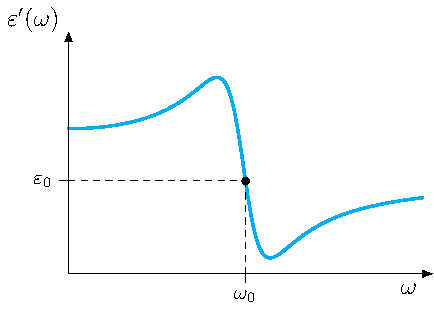
\includegraphics[width=\linewidth]{img/1/Epsilon_real.pdf}
        \end{subfigure}\hfil
        \begin{subfigure}[b]{0.45\linewidth}
            \centering
            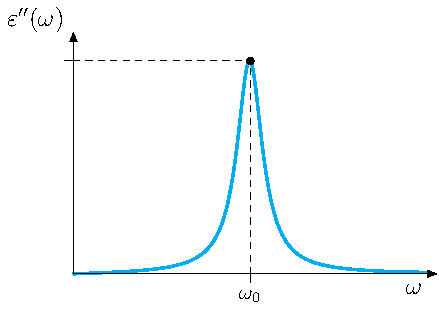
\includegraphics[width=\linewidth]{img/1/Epsilon_imag.pdf}
        \end{subfigure}
        \caption{Partes real e imaginária da permitividade efetiva $\epsilon(\omega)$.}
    \end{figure}

    \footnotetext{A componente $\epsilon'$ representa a permitividade sem perdas, i.e., $\epsilon' = \epsilon_0 \epsilon_r$. $\epsilon''$ é a componente imaginária da permitividade atribuída às cargas ligadas e relaxamento dipolar, que originam perdas de energia indistinguíveis das perdas devido à condução de cargas.}
\end{warning}

%//==============================--@--==============================//%
\subsubsection{Meio Condutor Dispersivo}

As propriedades de condutividade de um material são descritas pela lei de Ohm. Para derivar esta lei do nosso modelo simples, usamos a relação $\mathbf{J} = \rho \dot{\mathbf{r}}$, onde a densidade de carga de condução é $\rho = Ne$. Consequentemente,
$$
    \mathbf{\underline{J}} = \rho (j\omega\mathbf{\underline{r}}) = \frac{j\omega Ne^2}{m} \frac{1}{\omega_0^2 - \omega^2 + j\omega\Gamma}\, \mathbf{\underline{E}} \equiv \sigma(\omega)\mathbf{\underline{E}}
$$
e, portanto, identificamos a condutividade $\sigma(\omega)$:
$$
    \sigma(\omega) = \frac{j\omega Ne^2}{m} \frac{1}{\omega_0^2 - \omega^2 + j\omega\Gamma} = \frac{j\omega\epsilon_0\omega_p^2}{\omega_0^2 - \omega^2 + j\omega\Gamma}
    \overset{\substack{\text{para}\\\text{$\omega_0 = 0$}\vspace{1mm}}}{\:\implies}
    \sigma(\omega) = \frac{\epsilon_0 \omega^{2}_{p}}{\Gamma + j\omega}
    \quad \text{``modelo de Drude''}
$$
Notamos que $\sigma(\omega)/j\omega$ é essencialmente a suscetibilidade elétrica considerada anteriormente. De facto, temos $\mathbf{\underline{J}} = j\omega \mathbf{\underline{P}}$, e portanto, $\mathbf{\underline{P}} = \mathbf{\underline{J}}/j\omega = (\sigma(\omega)/j\omega) \mathbf{\underline{E}}$. Segue-se que $\epsilon(\omega) - \epsilon_0 = \sigma(\omega)/j\omega$, e
$$
    \epsilon(\omega) = \epsilon_0 + \frac{\epsilon_0\omega_p^2}{\omega_0^2 - \omega^2 + j\omega\Gamma} = \epsilon_0 + \frac{\sigma(\omega)}{j\omega}
$$

%//==============================--@--==============================//%
\subsection{Material Genérico} \label{sec:material-generico-dispersivo}

Para descrever um material com ambas as \underline{propriedades dielétricas e condutivas}, podemos tomar a suscetibilidade como a soma de dois termos, um que descreve as cargas polarizadas ligadas e o outro as cargas de condução livres. Assumindo parâmetros diferentes $\{ \omega_0, \omega_p, \Gamma \}$ para cada termo, obtemos a permitividade total:
$$
    \epsilon(\omega) 
    =
    \epsilon_0 \Big[ 1 + \chi_d(\omega) + \chi_c(\omega) \Big]
    =
    \epsilon_0 
    + 
    \frac{\epsilon_0 \omega_{dp}^2}{\omega_{d0}^2 - \omega^2 + j\omega \Gamma_d} 
    + 
    \frac{\epsilon_0 \omega_{cp}^2}{\omega_{c0}^2 - \omega^2 + j\omega \Gamma_c}
$$
Agrupando os dois primeiros termos em $\epsilon_d(\omega)$ e denotanto o terceiro por $\sigma_c(\omega)/j\omega$, obtemos a permitividade efetiva total do material:
$$
    \boxed{%
        \epsilon(\omega) = \epsilon_d(\omega) + \frac{\sigma_c(\omega)}{j\omega}
    }
    \quad \text{(permitividade efetiva total)}
$$

\begin{check}
    Semelhante a $\mathbf{\underline{D}}$ e $\mathbf{\underline{E}}$, a indução e o campo magnético estão ligados por uma permeabilidade magnética complexa $\mu(\omega)$ tal que $\mathbf{\underline{B}} = \mu(\omega)\mathbf{\underline{H}}$. Substituindo $\mathbf{\underline{D}} = \epsilon(\omega)\mathbf{\underline{E}}$ e $\mathbf{\underline{B}} = \mu(\omega)\mathbf{\underline{H}}$ nas equações macroscópicas de Maxwell, descobre-se que:
    $$
        \nabla \times \mathbf{\underline{E}} = -j\omega\mu(\omega)\mathbf{\underline{H}},
        \quad
        \nabla \times \mathbf{\underline{H}} = \mathbf{\underline{J}}_{ext} + j\omega\epsilon(\omega)\mathbf{\underline{E}}, 
    $$
    onde $\epsilon (\omega)$ é a permitividade complexa equivalente acima, que inclui as contribuições das correntes de condução e das correntes de polarização.
\end{check}

Admitindo $\epsilon_d(\omega) = \epsilon'_d(\omega) - j\epsilon''_d(\omega)$, como visto anteriormente, e assumindo que a condutividade $\sigma_c(\omega)$ é real para a gama de frequências de interesse, podemos definir $\epsilon(\omega) = \epsilon'(\omega) - j\epsilon''(\omega)$, onde:
$$
    \epsilon'(\omega) = \epsilon'_d(\omega), \qquad \epsilon''(\omega) = \epsilon''_d(\omega) + \frac{\sigma_c(\omega)}{\omega}
$$
Uma maneira conveniente de quantificar as perdas é através da tangente de perdas (\textit{loss tangent}) definida em termos das partes real e imaginária da permitividade efetiva:
$$
    \boxed{ \tan \theta = \frac{\epsilon''(\omega)}{\epsilon'(\omega)} } \quad \text{onde $\theta$ é o ângulo de perdas.}
$$
%//==============================--@--==============================//%